\subsubsection{Rancangan Detail Antarmuka Client}
\label{subsubsection:detail-client-interface}

Antarmuka \textit{client} bertanggung jawab untuk menyediakan akses ke sistem bagi pengguna. Antarmuka ini akan menyediakan fungsi yang dibutuhkan, yaitu \textit{read} dan \textit{write} data. Antarmuka ini juga dapat digunakan pengguna untuk melihat status sistem, seperti status \textit{Node}, status \textit{Cluster}, dokumentasi, dan informasi lainnya yang diperlukan. Antarmuka \textit{client} akan dibuat memanfaatkan protokol HTTP. Alasan dari pemilihan protokol HTTP adalah karena protokol ini sudah umum digunakan dan didukung oleh banyak bahasa pemrograman maupun alat. Selain itu, protokol HTTP juga mudah digunakan dan dapat diakses melalui berbagai platform, termasuk web browser. Dukungan alat terhadap protokol HTTP akan memudahkan pengembangan dan pengujian sistem. Rancangan antarmuka \textit{client} dapat dilihat pada gambar \ref{fig:client-interface-component}.

\begin{figure}[ht]
    \centering
    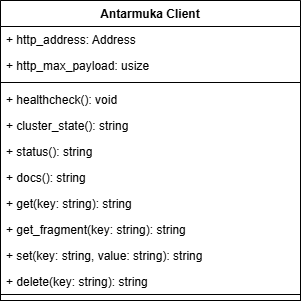
\includegraphics[width=0.45\textwidth]{resources/chapter-3/client-interface-component.png}
    \caption{Komponen Antarmuka Client}
    \label{fig:client-interface-component}
\end{figure}

Antarmuka tersebut akan terhubung pada \textit{endpoint} HTTP yang disediakan. Fungsi yang ada akan dieksekusi ketika \textit{request} diterima pada \textit{endpoint} yang sesuai.